
%%% Local Variables:
%%% TeX-master: t
%%% coding: utf-8
%%% mode: latex
%%% End:

\documentclass[notes]{beamer}
\usetheme{Boadilla}

\usepackage[utf8]{inputenc}
\usepackage[english]{babel}

\usepackage{graphicx}
\graphicspath{ {images/} }

\usepackage{xcolor}
\definecolor{light-gray}{gray}{0.90}
\makeatletter
\def\mathcolor#1#{\@mathcolor{#1}}
\def\@mathcolor#1#2#3{%
  \protect\leavevmode
  \begingroup
    \color#1{#2}#3%
  \endgroup
}
\makeatother


\usepackage{listings}
\lstdefinestyle{bnf}{
  mathescape,
  basicstyle=\footnotesize\ttfamily,
  breaklines=true
}

\usepackage{mathpartir}
\newcommand{\rulename}[1]{\textsc{\MakeLowercase{#1}}}
\newcommand{\derivRule}[3]{
  \inferrule*[Left=#1]{#3}{#2}
}
\newcommand{\derivTree}[3]{
  \inferrule*[Right=#1]{#3}{#2}
}

\title[Phometa]{\textbf{Phometa} --- a visualised proof assistant \\
       that builds a formal system and proves \\
       its theorems using derivation trees}
\author{Gun Pinyo}
\institute{Imperial College London}
\date{June 21, 2016}

\begin{document}

\frame{\titlepage}

\note{ Good morning everybody, today, it is an honour for me to present my
  dedicated proof assistant named ``Phometa'' which is a tool that can be used
  to construct a formal system and its theorems.
}

\begin{frame}
\frametitle{Derivation systems can reason many formal systems.}
$$
\derivTree{mult-intro,leftskip=6em}{(((w \times x) + (w \times y)) \times z) =
                         ((w \times (x + y)) \times z)}
  { \derivTree{eq-symm}{((w \times x) + (w \times y)) =
                         (w \times (x + y))}
    { \derivTree{dist-left}{(w \times (x + y)) = ((w \times x) + (w \times y))} { }
    }
   \\ \\ \\
    { \derivTree{eq-refl}{z = z}{ }
    }
  }
$$
\vspace{1ex}
$$
\derivTree{and-intro,leftskip=6em}{p, p \rightarrow q \vdash p \wedge q}
  { \derivTree{ass}{p, p \rightarrow q \vdash p} { }
    \\
    \derivTree{imply-elim}{p, p \rightarrow q \vdash q}
    { \derivTree{ass}{p, p \rightarrow q \vdash p \rightarrow q} { }
      \\
      \derivTree{ass}{p, p \rightarrow q \vdash p} { }
    }
  }
$$
\vspace{1ex}
$$
\derivTree{arrow-elim,leftskip=6em}{y : A \vdash (\lambda x . x) y : A}
  { \derivTree{arrow-intro}{y : A \vdash \lambda x . x : A \rightarrow A}
    { \derivTree{assumption}{y : A, x : A \vdash x : A} { }
    }
  \\ \\ \\ \\
    \derivTree{assumption}{y : A \vdash y : A}{ }
  }
$$
\end{frame}

\note{ Derivation system is capable to reason about many formal systems. For
  example we can prove that (TODO) is valid by creating a derivation tree using
  grammars and derivation rules of simple arithmetic. The similar things happen
  in propositional logic and typed lambda calculus as well.

  However, there is no such a framework that manage to handle a derivation
  system in general way. This motivated me to build ``Phometa'' which is a proof
  assistant that can encode Simple Arithmetic, Propositional Logic, Typed Lambda
  Calculus and any arbitrary formal system that can be reasoned using a
  derivation system.
}

\begin{frame}
\frametitle{Screenshot of  ``Phometa'' in action}
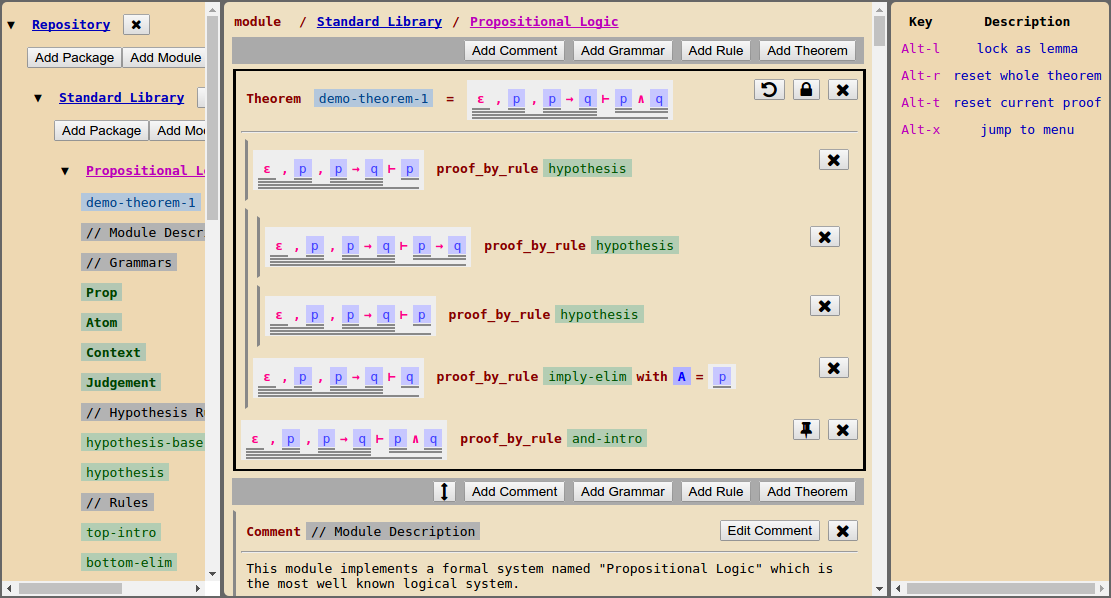
\includegraphics[width=\linewidth,height=\textheight,keepaspectratio]{demo-1}
\end{frame}

\note{ In this presentation, I will use Propositional Logic as an example of a
  formal system to explain about Phometa. [point to screen] Here is a screenshot
  that shows Phometa in action, you can see that we have been successfully prove
  that $p \wedge q$ holds under an assumption that $p$ and $p \rightarrow q$
  hold, this is the same tree as one of derivation tree on the previous slide
  [swap to previous slide to show them again and swap back]. Please notice that
  the tree is similar to a traditional one but no longer suffer the fact that
  its width grows exponentially to its height. We also exploit the power of
  visualisation such as using underlines to group sub-terms instead of
  brackets.}

\begin{frame}[fragile]
\frametitle{Formal system ingredient - Grammar (Backus-Nour Form)}
\begin{lstlisting}[style=bnf]
<Prop> ::= `$\top$' | `$\bot$' | <Atom>
         | `('<Prop> `$\wedge$' <Prop>`)'
         | `('<Prop> `$\vee$' <Prop>`)'
         | `( $\neg$' <Prop>`)'
         | `('<Prop> `$\rightarrow$' <Prop>`)'
         | `('<Prop> `$\leftrightarrow$' <Prop>`)'
         | meta-variables comply with regex
             /[A-Z][a-zA-Z]*([1-9][0-9]*|'*)/
\end{lstlisting}
\end{frame}

\note{As I told you that Phometa is capable to implement arbitrary formal
  system, so there is a method to this. For example, we can }



\begin{frame}
\frametitle{Grammar (Backus-Nour Form) (Continue).}
\end{frame}

\begin{frame}
\frametitle{Underline instead of brackets.}
\end{frame}

\begin{frame}
\frametitle{Rule (Derivation Rule).}
\end{frame}

\begin{frame}
\frametitle{Theorem (Derivation Tree).}
\end{frame}

\begin{frame}
\frametitle{Demonstration.}

\begin{itemize}
\item show overall user interface
\item construct root term $p, p \rightarrow q \vdash p$
\item write a theorem to prove $p, p \rightarrow q \vdash p$
\item write a theorem to prove $\vdash (p \rightarrow q) \vee (q \rightarrow p)$
\item add extend propositional logic to support equivalent
\end{itemize}

\end{frame}

\begin{frame}
\frametitle{Cascade premise.}
\end{frame}

\begin{frame}
\frametitle{Meta reduction.}
\end{frame}

\begin{frame}
\frametitle{Elm language, Signal, and MCV architecture (if have time).}
\end{frame}

\begin{frame}
\frametitle{Evaluation (if have time).}
\end{frame}

\end{document}
